\documentclass{beamer}
%\usepackage[utf8]{inputenc}
\usepackage{lipsum}
\usepackage[mathscr]{euscript}
\usepackage{amsmath,amssymb}
%\usepackage{enumitem} %for beggining item with letter
\usepackage[linesnumbered,ruled]{algorithm2e}
%\usepackage[justification=centering]{caption}
%tensors
\newcommand\sdots{\!\hbox to 1em{.\hss.\hss.}}

\newcommand{\mX}{\mathcal X}
\newcommand{\mC}{\mathcal C}
\newcommand{\mD}{\mathcal D}
\newcommand{\mY}{\mathcal Y}
\newcommand{\mS}{\mathcal S}
\newcommand{\mB}{\mathcal B}
\newcommand{\mA}{\mathcal A}
\newcommand{\mG}{\mathcal G}
\newcommand{\mP}{\mathcal P}
\newcommand{\mZ}{\mathcal Z}
\newcommand{\mM}{\mathcal M}
\newcommand{\mL}{\mathcal L}
\newcommand{\mE}{\mathcal E}
\newcommand{\mV}{\mathcal V}
\newcommand{\mH}{\mathcal H}
\newcommand{\mJ}{\mathcal J}
\newcommand{\mW}{\mathcal W}
% estimated(widehat) tensors
\newcommand{\mhM}{\mathcal{ \widehat M}}
\newcommand{\mhL}{\mathcal{ \widehat L}}
\newcommand{\mhB}{\mathcal{ \widehat B}}
\newcommand{\mhZ}{\mathcal{ \widehat Z}}
\newcommand{\mhV}{\mathcal{ \widehat V}}
% mean(widehat) tensors
\newcommand{\mbX}{\mathcal{ \bar X}}
\newcommand{\mbY}{\mathcal{ \bar Y}}
%bold
\newcommand{\bX}{\boldsymbol{X}}
\newcommand{\bx}{\boldsymbol{x}}
\newcommand{\bz}{\boldsymbol{z}}
\newcommand{\bY}{\boldsymbol{Y}}
\newcommand{\bE}{\boldsymbol{E}}
\newcommand{\bc}{\boldsymbol{c}}
%operators
\DeclareMathOperator{\tr}{tr}
\DeclareMathOperator{\etr}{etr}
\DeclareMathOperator{\vecc}{vec}
\DeclareMathOperator{\vech}{vech}
\DeclareMathOperator{\N}{\mathcal N}
\DeclareMathOperator{\CN}{\mathcal{CN}}
\DeclareMathOperator{\I}{I}
\DeclareMathOperator*{\circs}{\circ}
\DeclareMathOperator*{\argmax}{arg\,max}
\DeclareMathOperator*{\argmin}{arg\,min}

%widehat matrices

\newcommand{\hM}{ \widehat M}
\newcommand{\hL}{ \widehat L}
\newcommand{\hSigma}{ \widehat \Sigma}

%enie
\newcommand{\gn}{\~{n}}

\newtheorem{defn}{Definition}[section] % definition numbers are dependent on theorem numbers
\newtheorem{thm}{Theorem}[section] % reset theorem numbering for each chapter
\newtheorem{cor}{Corollary}[section] % reset theorem numbering for each chapter
%\newtheorem{lemma}{Lemma}[section] % reset theorem numbering for each chapter
\newtheorem{property}{Properties}[section] % definition numbers are dependent on theorem numbers





%%%%%%%%%%%%%%%%%%%%%%%%%%%%%%%%%%%%%%%
%%%%%%%%%% BEAMER STUFF %%%%%%%%%%%%%%%
%%%%%%%%%%%%%%%%%%%%%%%%%%%%%%%%%%%%%%%

\mode<presentation>{
  \usetheme{Boadilla}      % or try Darmstadt, Madrid, Warsaw, ...
  \usecolortheme{sidebartab} % or try albatross, beaver, crane, ...
  \usefonttheme{serif}  % or try serif, structurebold, ...
  \setbeamertemplate{navigation symbols}{}
  \setbeamertemplate{caption}[numbered]
} 
\usepackage[english]{babel}
\usepackage[utf8x]{inputenc}
\usepackage{xcolor}
\usepackage{listings}
\usepackage{amsthm}
\usepackage{amsmath}
\usepackage{graphicx}
\usepackage{bm}
\lstset{
    language=[LaTeX]TeX,
    breaklines=true,
    basicstyle=\tt\scriptsize,
    %commentstyle=\color{green}
    keywordstyle=\color{blue},
    %stringstyle=\color{black}
    identifierstyle=\color{magenta},
}









\title[]{Tensor Data Analysis Overview}
\author{Carlos Llosa}
\institute{STAT 680 lecture \\ November 08,2021 }
\date{}
\AtBeginSection[]
{
  \begin{frame}<beamer>
    \frametitle{Outline}
    \tableofcontents[currentsection,currentsubsection]
  \end{frame}
}














\begin{document}













\begin{frame}
  \titlepage
  \centering
  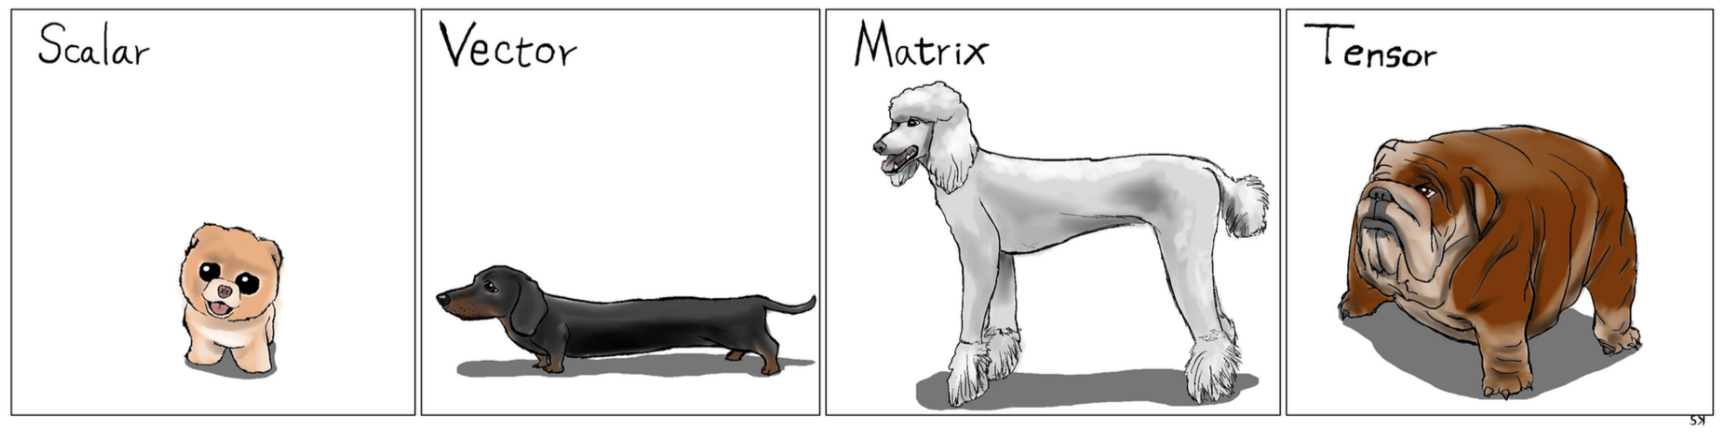
\includegraphics[height = 2.5cm]{figures/tensordogs.png}
\end{frame}

\begin{frame}{Outline}
  \tableofcontents
\end{frame}























\section{Tensors when the observations are scalars}

\begin{frame}{Human Mortality Database }
  \centering
  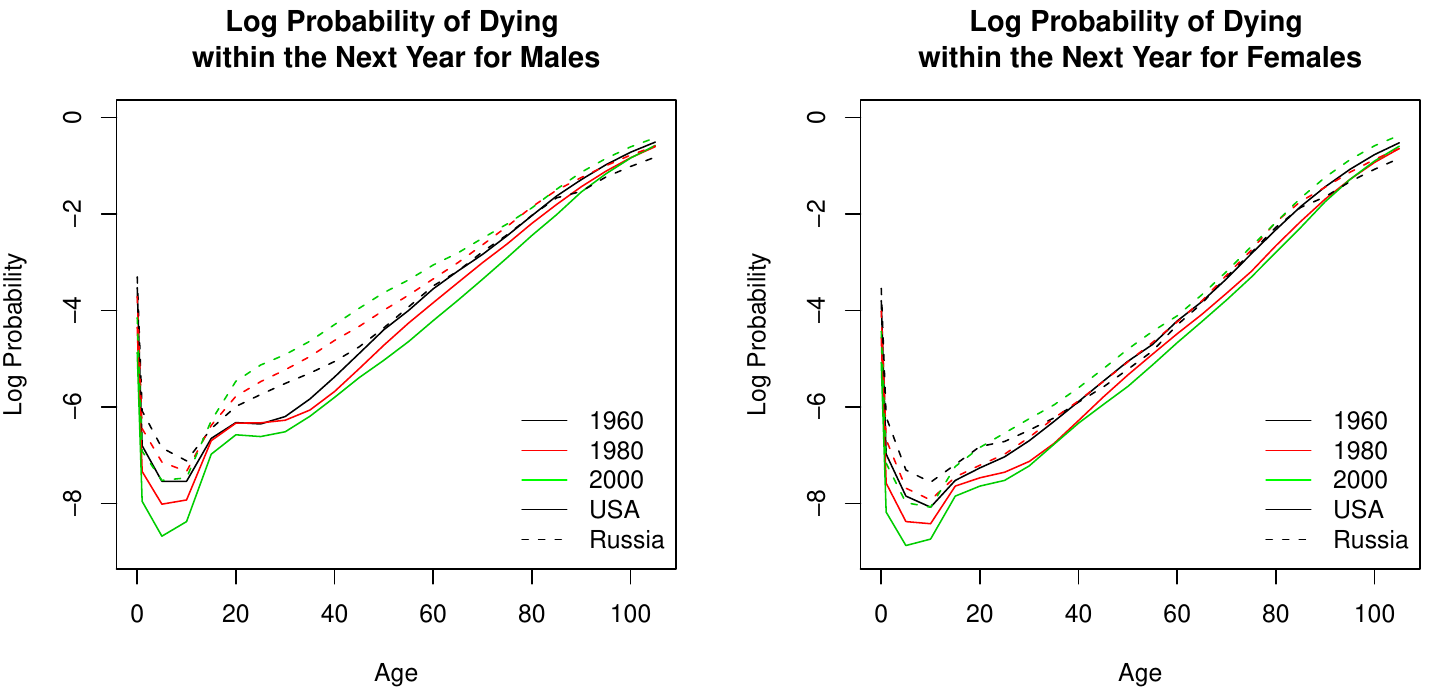
\includegraphics[height = 4cm]{figures/human-mortality.png}

Tensor form along different factors:
\begin{itemize}
\item 38 countries
\item 23 age levels (0,1, then every 5 years)
\item 9 time periods (1960-2000 every 5 years)
\item 2 sexes
\end{itemize}
$39\times 23\times 9\times 2$ array!
\end{frame}






\begin{frame}{Factorial Designs }

Cell means ANOVA:
\quad
$
y_{ijklm} = \mu_{ijkl} + e_{ijklm}
$

\begin{itemize}

\item In STAT 500-510 deep interactions:
$$
\mu_{ijkl} = \alpha_i + \beta_j + \eta_k + \gamma_l +
\alpha\beta_{ij}+
\alpha\eta_{ik}+
\alpha\gamma_{il}+
\beta\eta_{jk}+
\beta\gamma_{jl}+
\eta\gamma_{kl}+$$$$
(\alpha\beta\eta)_{ijk}+
(\alpha\beta\gamma)_{ijl}+
(\alpha\eta\gamma)_{ikl}+
(\beta\eta\gamma)_{jkl}+
(\alpha\beta\eta\gamma)_{ijkl}
$$
\item we could do
$
\mu_{ijkl} = \langle\mX_{ijkl},\mB\rangle,
$
where
$$
\mX_{i^*j^*k^*l^*} = \begin{cases} 
      1 & if (i,j,k,l)=(i^*,j^*,k^*,l^*)  \\
      0 & otherwise
   \end{cases}
$$
Then $\mB$ is an array that contains all the relevant means and deep interactions!
\end{itemize}

\end{frame}





\begin{frame}{Tensor Regression}
\begin{itemize}
\item Simple linear regression
		$$y_i = \beta x_i + \epsilon_i, \quad \epsilon_i \overset{iid}{\sim} \N(0,\sigma^2)$$
\item Multiple linear regression		
$$  y_i = \bm{\beta}' \bm{x_i} + \epsilon_i, \quad \epsilon_i \overset{iid}{\sim} \N(0,\sigma^2)$$
\item Tensor regression
$$  y_i = \langle \mB, \mX_i\rangle + \epsilon_i, \quad \epsilon_i \overset{iid}{\sim} \N(0,\sigma^2)$$
  	\end{itemize}
\end{frame}

\section{Tensors  with multivariate observations}

\begin{frame}{Brain Imaging Data (Yamashita et.al 19)}
  \centering
  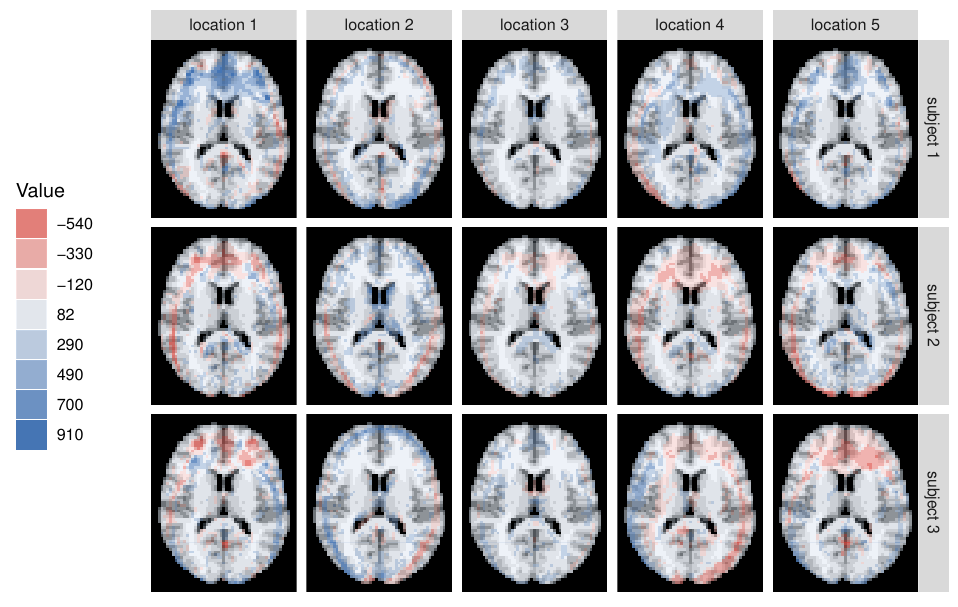
\includegraphics[height = 5cm]{figures/traveling-subjects.png}
  
tensor form along multiple factors and spatial dimensions!
\begin{itemize}
\item 9 subjects traveled to 12 imaging centers
\item 3 repetitions of  240 time-steps each
\item brain images of size $73\times 73\times 61$
\end{itemize}
$73\times 73\times 61\times 240\times 9\times 12\times 3$ array!
\end{frame}



\begin{frame}{Multivariate Regression}
	\begin{itemize}
			\item Multivariate Multiple Linear Regression
			$$ \bm{y}_i = B \bm{x_i} + \boldsymbol{\epsilon}_i, \quad \boldsymbol{\epsilon}_i \overset{iid}{\sim} \N_m(0,\Sigma),$$
\item Matrix-variate Regression (Ding and Cook, 2018, JRSSB)
			$$ Y_i = B_1 X_i B_2^\intercal + E_i, \quad E_i \overset{iid}{\sim} \N_{m_1,m_2}(0,\Sigma_1,\Sigma_2),$$
\item Multilinear Tensor Regression  (Hoff, 2015,  Ann. Appl. Stat)
$$
 \mY_i = [\![ \mX_i; B_1, \hdots,B_p  ]\!]	+\mE_i
, \quad \mE_i \overset{iid}{\sim} 
\N_{m_1, \hdots, m_p}(0,\Sigma_1,\hdots, \Sigma_p),
$$
\end{itemize}
\end{frame}
\subsection{Kronecker Separability for Higher Order Normality}



\begin{frame}{The Matrix Normal Distribution}
\begin{itemize}
\item S. N. Roy wrote its pdf in 1957
\item A matrix follows a normal distribution if its vectorization follows a multivariate normal distribution
\item Without any constraint on the covariance matrix, this leads to overfitting 
\item Kronecker separability is an intuitive constraint
\end{itemize}
Definition:
$$
X \sim \N_{m_1,m_2}\big(M,\Sigma_1, \Sigma_2 \big)
  \iff \vecc(X) \sim \N_{m_1 \times m_2} \big(\vecc(M), \Sigma_2 \otimes \Sigma_1 \big)
$$
\begin{center}
dimensionality reduction:

$ \big[(m_1\times m_2 +1 ) (m_1\times m_2) \big]/2 \hspace{0.5cm} \rightarrow  \hspace{0.5cm} 
(m_1+1)\times m_1/2 + (m_2+1)\times m_2/2$
\end{center} 
\end{frame}

\begin{frame}{The Tensor Normal Distribution}
\begin{itemize}

\item A tensor follows a normal distribution if its vectorization follows a multivariate normal distribution

\item The assumption of kronecker separability can be extended to higher order tensors

\item Vectorization is usually defined in reverse lexicographic order to avoid an inconsistency with matrix vectorization
\end{itemize}
Definition:\\
$
\hspace{1cm} \mX \sim \N_{m_1,\hdots, m_p}\big(\mM \hspace{0.15cm},\Sigma_1,\hdots,\Sigma_p\big)
  $\vspace*{-0.5cm} $$
 \hspace*{2cm} \iff \vecc(\mX) \sim \N_{m_1 \times\hdots\times m_p} \big(\vecc(\mM), \bigotimes_{i=p}^1 \Sigma_i \big)
\vspace*{-0.5cm}$$


\end{frame}

\begin{frame}{Comparisons between tensor normal distributions}

\begin{itemize}
\item Bivariate normal distribution:  $\bm{x} \sim  \N_2(\boldsymbol{\mu},\Sigma),\quad \Sigma[i,j] = \sigma_{ij} $
$$
\begin{bmatrix}
x_1 \\ x_2 
\end{bmatrix}
 \sim \N_2 \Big(  
\begin{bmatrix}
\mu_1 \\ \mu_2
\end{bmatrix},\quad
\begin{bmatrix}
  \sigma_{11} & \sigma_{12} \\ \sigma_{21} & \sigma_{22}
\end{bmatrix}
\Big)
$$

\item Matrix normal distribution: $X \sim \N_{3,2}(M,\Sigma_1,\Sigma),\quad \Sigma[i,j] = \sigma^2_{ij} $
$$
\vecc(X)=
\begin{bmatrix}
 \boldsymbol{x_1} \\ \boldsymbol{x_2} 
\end{bmatrix}  \sim \N_{3 \times 2} \Big(  
\begin{bmatrix}
\boldsymbol{\mu_1} \\ \boldsymbol{\mu_2}
\end{bmatrix},\quad
\begin{bmatrix}
 \sigma_{11}\Sigma_1 & \sigma_{12}\Sigma_1 \\ \sigma_{21}\Sigma_1 & \sigma_{22}\Sigma_1
\end{bmatrix}
\Big).
$$

\item Third order tensor normal distribution: $\mX \sim \N_{3,2,2} (\mM,\Sigma_1,\Sigma_2,\Sigma)$
$$
\hspace*{0.5cm}\vecc(\mX)=
\begin{bmatrix}
 \vecc{\mX(:,:,1)} \\ \vecc{\mX(:,:,2)}
\end{bmatrix}  \hspace*{8cm} \vspace*{-0.3cm}$$
$$ \hspace*{1cm} \sim \N_{3 \times 2 \times 2} \Big(  
\begin{bmatrix}
 \vecc{\mM(:,:,1)} \\ \vecc{\mM(:,:,2)}
\end{bmatrix},
\begin{bmatrix}
 \sigma_{11}\Sigma_2 \otimes \Sigma_1 & \sigma_{12}\Sigma_2 \otimes \Sigma_1 \\ \sigma_{21}\Sigma_2 \otimes \Sigma_1 & \sigma_{22}\Sigma_2 \otimes \Sigma_1
\end{bmatrix}
\Big).
$$
\end{itemize}




\end{frame}


\begin{frame}{Back to Matrix-Variate Regression}
	\begin{center}
			$$ Y_i = B_1 X_i B_2^\intercal + E_i, \quad E_i \overset{iid}{\sim} \N_{m_1,m_2}(0,\Sigma_1,\Sigma_2),$$
	\end{center}
	\small
	\begin{itemize}
	\item MLE under fixed $(B_2,\Sigma_2)$:\\
	Let $H_1 = \sum_{i=1}^n X_iB_2'\Sigma_2^{-1}B_2X_i'$, then
	$$
	 \begin{cases} 
       \widehat{B}_1 = (\sum_{i=1}^n Y_i\Sigma_2^{-1}B_2X_i')H_1^{-1}
        \\
      \widehat{\Sigma}_1 = \sum_{i=1}^n Y_i\Sigma_2^{-1}Y_i' - \widehat{B}_1 H_1\widehat{B}_1 '
   \end{cases}
   $$
   \item MLE under fixed $(B_1,\Sigma_1)$:\\
	Let $H_2 = \sum_{i=1}^n X_i'B_1'\Sigma_1^{-1}B_1X_i$, then
	$$
	 \begin{cases} 
       \widehat{B}_2 = (\sum_{i=1}^n Y_i'\Sigma_1^{-1}B_1X_i)H_2^{-1}
        \\
      \widehat{\Sigma}_2 = \sum_{i=1}^n Y_i'\Sigma_1^{-1}Y_i - \widehat{B}_2 H_2\widehat{B}_2 '
   \end{cases}
   $$
   \item Block relaxation algorithm!!!
   \item You should avoid this model $\rightarrow$ tensor on tensor regression!
	\end{itemize}
\end{frame}


\section{Low-Rank Formats}





%%%%%%%%%%%%%%%%%%%%%%%%%%%%%%%%%%%%%%%%%%%%%%%

\begin{frame}{The Tucker (TK)  Format}
\vspace*{-0.3cm}


\begin{center}
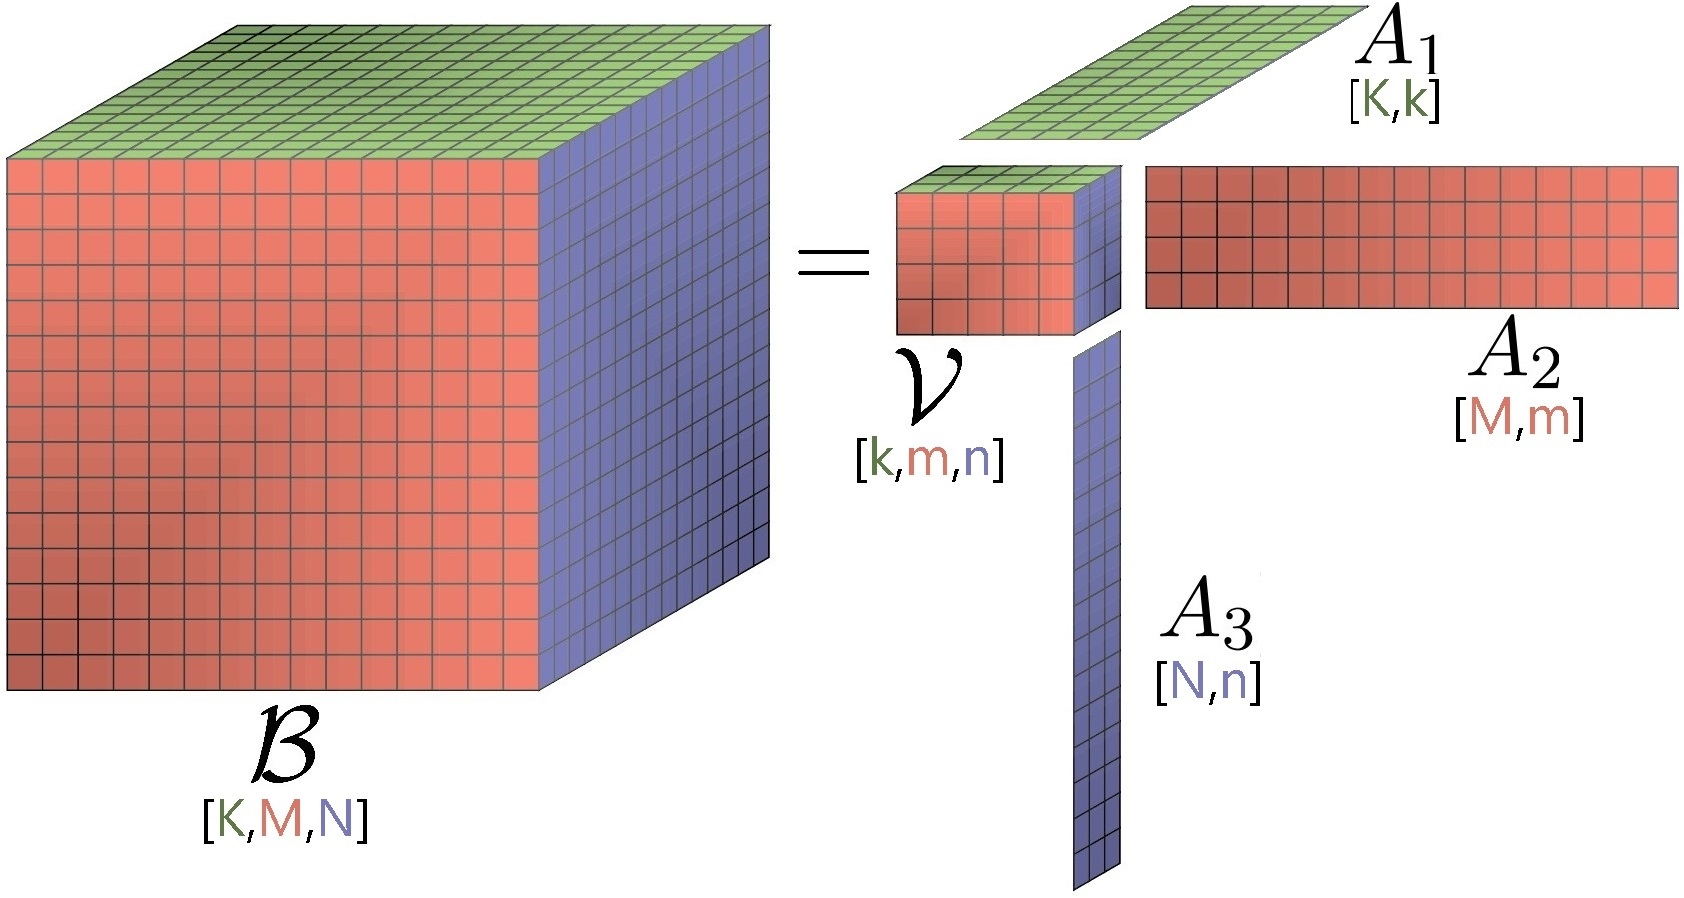
\includegraphics[width=6cm]{figures/tucker-paper.jpg}
\end{center}
\vspace*{-0.5cm}
$$
\mB = [\![ \mV; A_1,A_2,A_3]\!]
$$

\begin{itemize}
\item Unconstrained $\mB\in \mathbb{R}^{15\times 15\times 15}$ has 3,375 parameters
\item Constrained to a Tucker format of rank (3,4,5) leads to only 240
\end{itemize}
\end{frame}





%%%%%%%%%%%%%%%%%%%%%%%%%%%%%%%%%%%%%%%%%%%%%%%


\begin{frame}{The Canonical (CP)  format}

\begin{center}
     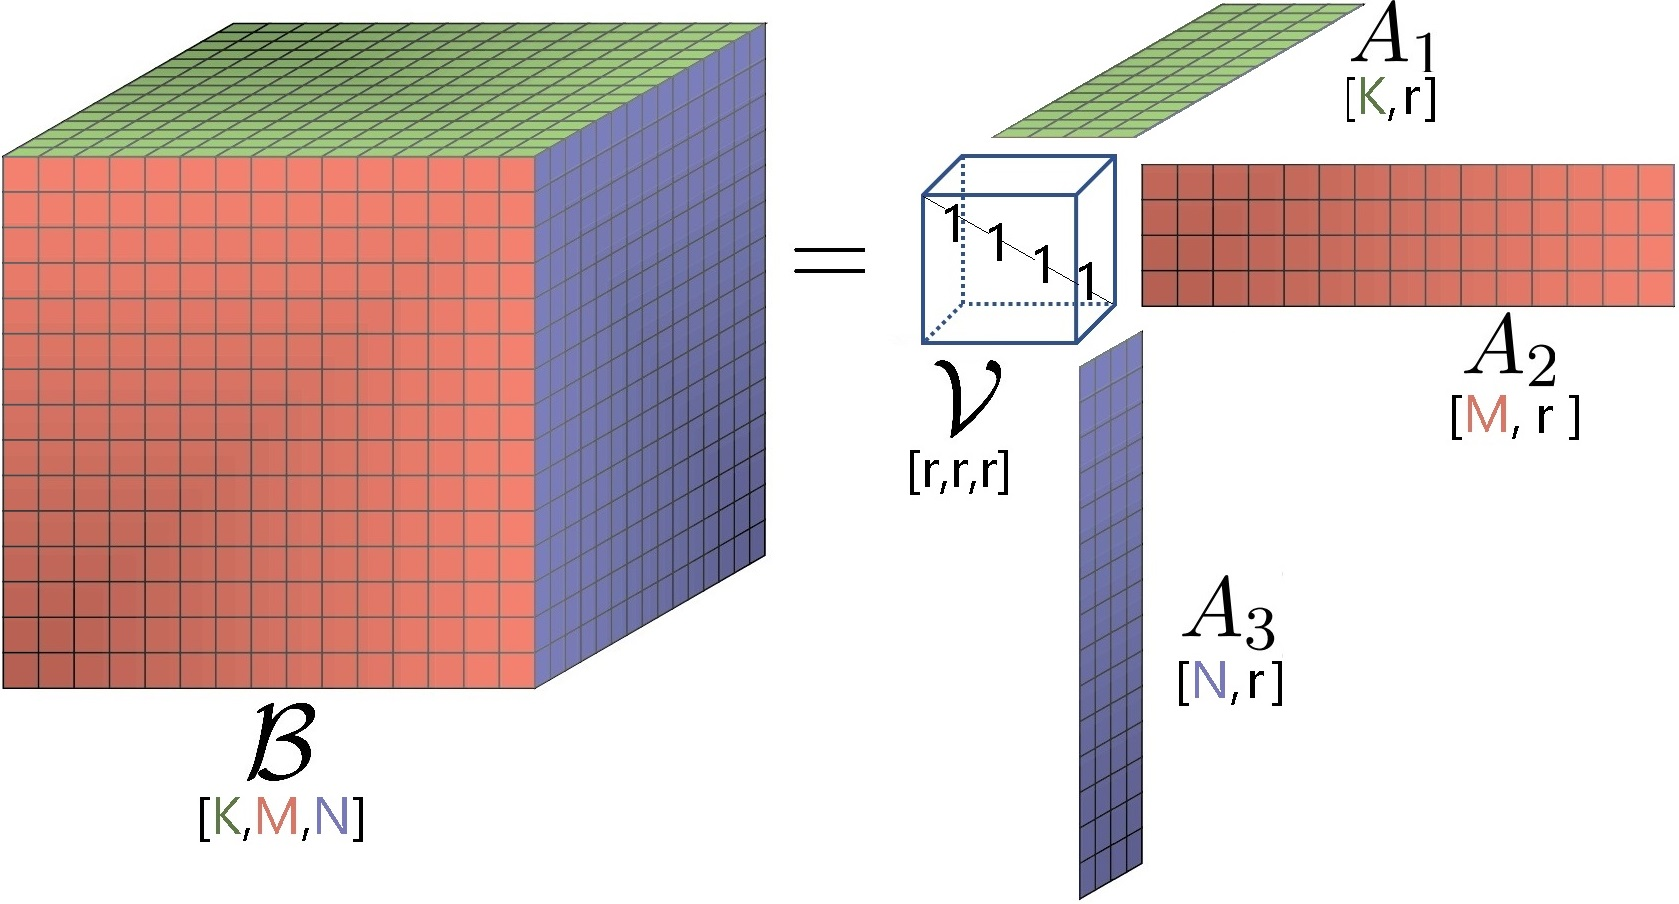
\includegraphics[width=6cm]{figures/CPpaper.jpg}
\end{center}
\vspace*{-0.5cm}
$$\mB = [\![ A_1,A_2,A_3]\!]$$ 
\vspace*{-0.5cm}
\begin{itemize}
\item Special case when core $\mV$ is \textit{diagonal}
\item Unconstrained $\mB$ has 3,375 parameters
\item Constrained to a CP format of rank 4 leads to only 180
\end{itemize}

\end{frame}


%%%%%%%%%%%%%%%%%%%%%%%%%%%%%%%%%%%%%%%%%%%%%%%



%%%%%%%%%%%%%%%%%%%%%%%%%%%%%%%%%%%%%%%%%%%%%%%



\begin{frame}{The Tensor Ring (TR)  Format}

 \begin{center}
     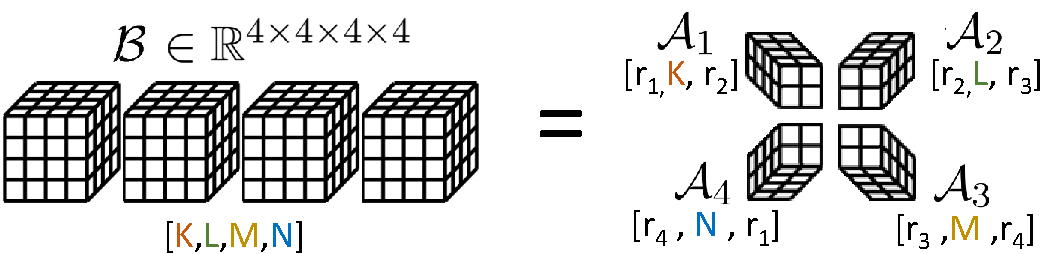
\includegraphics[width=8cm]{figures/TR-nonetwork-crop.pdf}
\end{center}
$$
\mB = \tr\left(
\mA_1 \!\times^1\!\!
\mA_2 \!\times^1\!\!
\mA_3 \!\times^1\!\!
\mA_4
\right)
$$

 \begin{itemize}
\item Referred to matrix product state (MPS) in many-body physics
\item Unconstrained $\mB$ has 256 parameters
\item Constrained to a TR format of rank (2,2,2,2) leads to only 64
\end{itemize}

\end{frame}


\begin{frame}
\begin{block}{Tensor-on-Tensor Regression:}
\begin{center}
$\mY_{i} =  \langle \mX_{i}|\mB \rangle + \mE_{i}
,\quad  \mE_{i}\overset{iid}{\sim} \N_{m_1,m_2\hdots,m_p}(0, \sigma^2 \Sigma_1,\Sigma_2,\hdots,\Sigma_p),$
\\\vspace*{.1cm}
$\mX_i \in \mathbb{R}^{h_1\times h_2\times\hdots \times h_l}
,\quad
\mY_i \in \mathbb{R}^{m_1\times m_2\times\hdots \times m_p},$
\\\vspace*{.1cm}
$\mB \in \mathbb{R}^{h_1\times h_2\times\hdots \times h_l\times m_1\times m_2\times\hdots \times m_p}.$
\end{center}
\end{block}

\begin{itemize}
\item Multilinear Tensor Regression is the case where $\mB$ has an OP format $\mB_{OP} = \circ[\![M_1,M_2,\dots,M_p]\!]$ because
$$
 \langle \mX_{i}|\mB_{OP} \rangle 
 =
 [\![\mX_i; M_1,M_2,\dots,M_p]\!].
$$

\item You can instead do a CP, TR or TK format!
\end{itemize}

\end{frame}

\end{document}
























